
\section{Force and Motion I\footnote{
1990-93 Dept. of Physics and Astronomy, Dickinson College. Supported by FIPSE
(U.S. Dept. of Ed.) and NSF. Portions of this material may have been modified
locally and may not have been classroom tested at Dickinson College.
}}

\makelabheader %(Space for student name, etc., defined in master.tex or labmanual_formatting_commands.tex)

\medskip
\textbf{Objectives }

\begin{itemize}[nosep]
\item To understand the relationship between forces applied to an object and its motions. 
\item To find a mathematical relationship between the force applied to an object and its acceleration.
\end{itemize}
\textbf{Overview }

In the previous labs, you used motion sensors and smart carts to display position-time,
velocity-time and acceleration-time graphs for different objects. You were not concerned about how you got the objects to move, i.e., what forces (pushes or pulls) acted on the objects. From your experiences, you know that force and motion are related in some way. To start your bicycle moving, you must apply a force to the pedal. To start up your car, you must step on the
gas pedal to get the engine to apply a force to the road through the tires.

But exactly how is force related to the quantities you used in the previous
unit to describe motion: position, velocity and acceleration? In this unit you
will pay attention to forces and how they affect motion. 
%You will apply forces
%to a cart, and observe the nature of its resulting motion graphically with a
%motion detector.

\medskip
\textbf{Apparatus} 

\begin{itemize} [nosep]
\item \textit{Capstone} software (\filename{V\_A\_F\_Graphs.cap} experiment file)
\item CS2000 compact scale
\item Dynamics track
\item Hanging masses
\item Pulley with clamp
\item String
\item Wireless smart cart
\end{itemize}
\textbf{Measuring Forces} 

In this investigation you will use a force sensor (built in to the smart cart) to measure forces. The force sensor puts out a voltage signal proportional to the force applied to the arm of the sensor. Physicists have defined a standard unit of force called the newton, abbreviated N. For your work on forces and the motions they cause, it will be more convenient to have the force sensor read directly in newtons rather than voltage. 
%Before the force probe is used it must be calibrated. Before calibrating the force probe, open the 

Open the \filename{V\_A\_F\_Graphs.cap} file in the \filename{\coursefolder} folder. Turn on the cart at your station and connect it to the computer via Bluetooth. At the beginning of each experiment, the measurements from the built-in acceleration and forces sensors may not be zero when the acceleration or force is actually zero. To tare the sensors, select the desired sensor (either the \textbf{Smart Cart Acceleration Sensor} or the \textbf{Smart Cart Force Sensor}) in the \textbf{Controls} palette and then click \textbf{Zero Sensor Now}. When taring the sensors, the cart should be at rest and there should be no applied force on the hook.
%To calibrate the force probe, see \textit{Calibrating Force Sensors} in \textbf{Appendix \ref{capstone}: Capstone}.

%\pagebreak[2]
%\textbf{Motion and Force} 
%
%Now you can use the force probe to apply measured amounts of force to an object.
%You can also use the motion detector, as in the previous units, to examine the
%motion of the object. In this way you will be able to establish the relationship
%between motion and force.
%\vspace{10mm}

\textbf{Activity 1: Pushing and Pulling a Cart} 

In this activity you will move a cart by pushing and pulling it with your hand and measure the force exerted on it, as well as the cart's velocity and acceleration. 
%Then you will be able
%to look for relationships between the applied force and the motion quantities,
%to see which is (are) related to force.

%\vspace{-0.2cm}
%{\par\centering 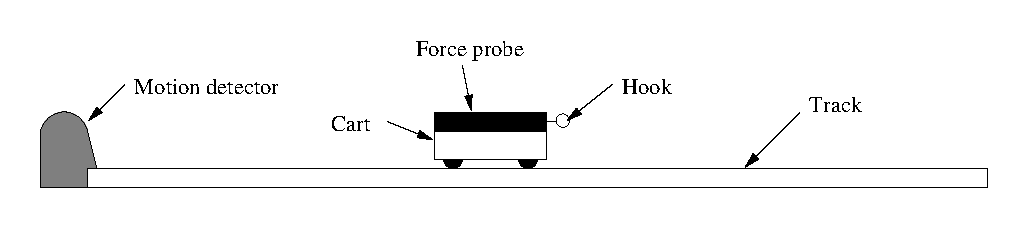
\includegraphics{force1/force1_fig1.eps} \par}
%{\par\centering 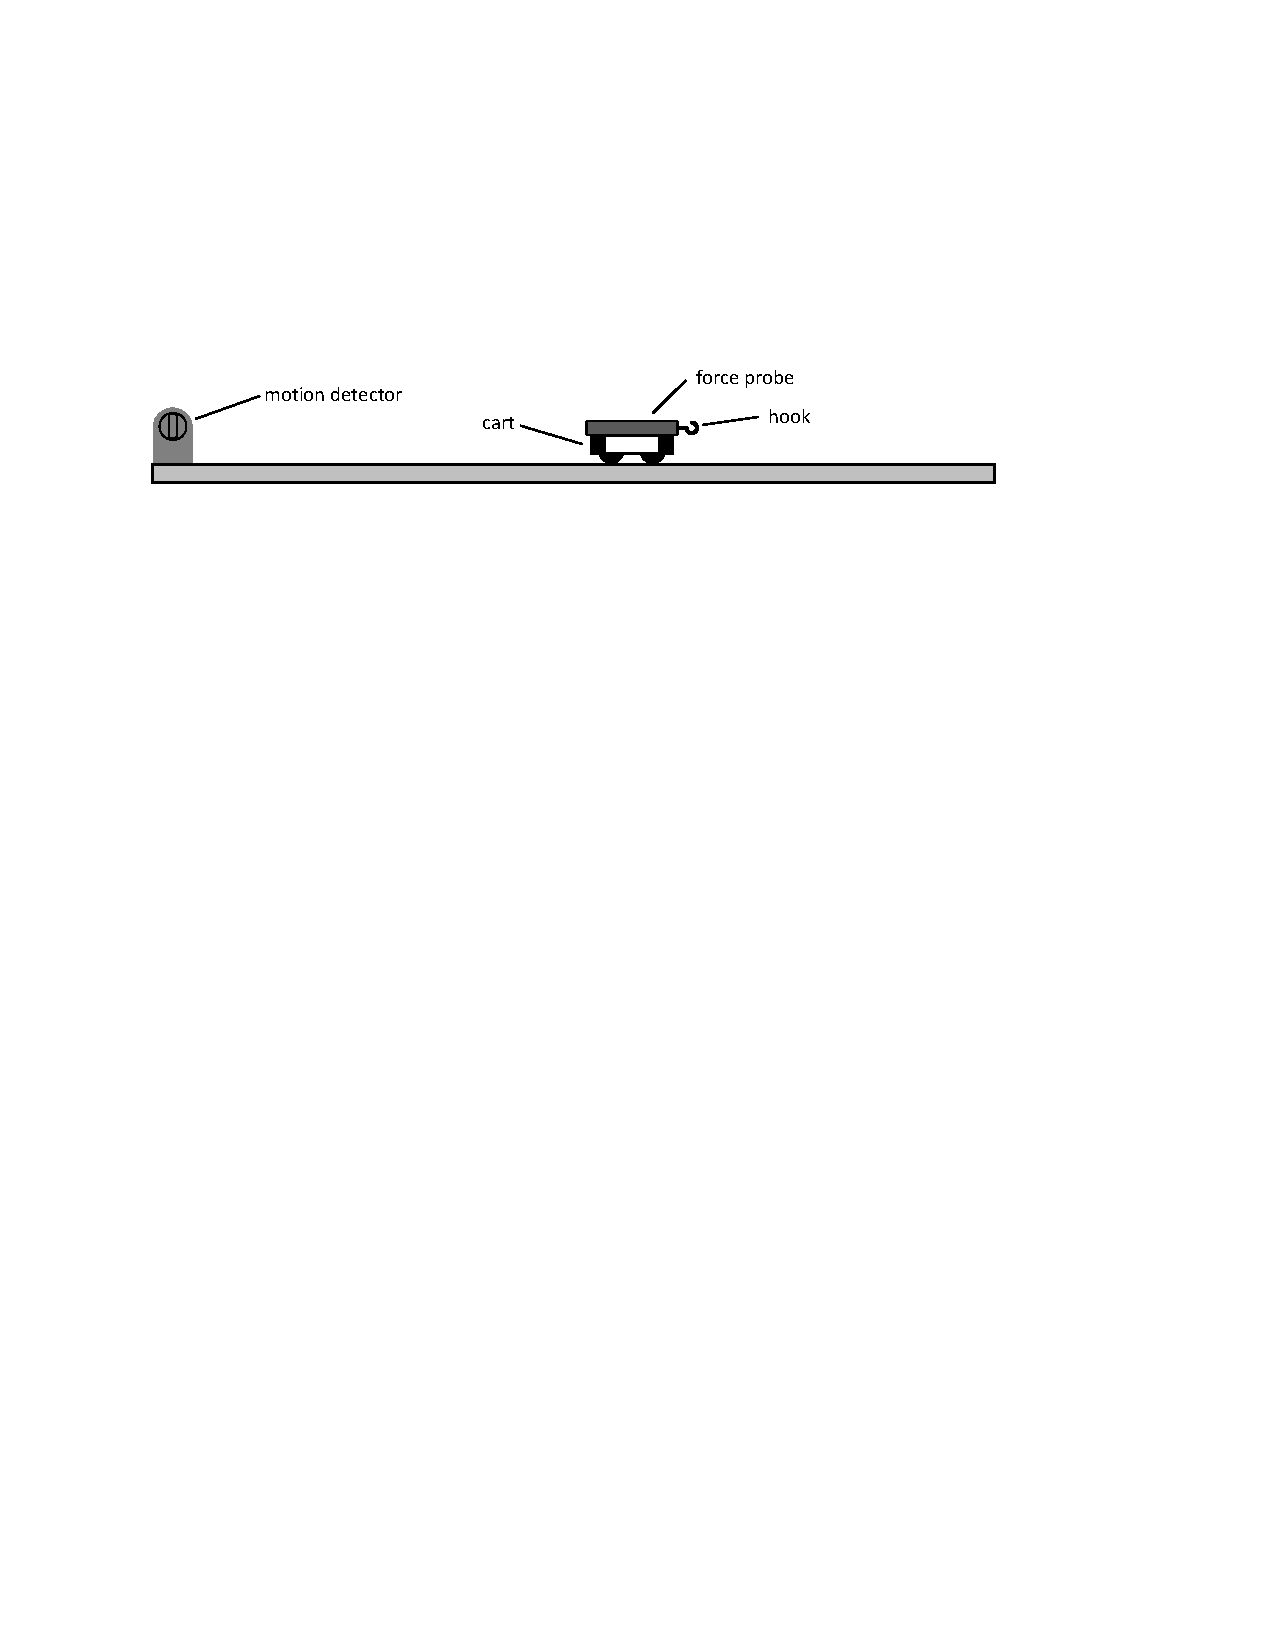
\includegraphics{force1/cart_and_sensors.pdf} \par}

(a) Measure the mass of the cart (using the compact scale) and record the result below.

\answerspace{10mm}

(b) Place the cart on the level track.  Suppose you were to grasp the hook on the cart (which is attached to the force sensor) and move the cart forwards and backwards. Would either the
velocity or the acceleration graph look like the force graph?
%\begin{figure}[t]
%{\par\centering 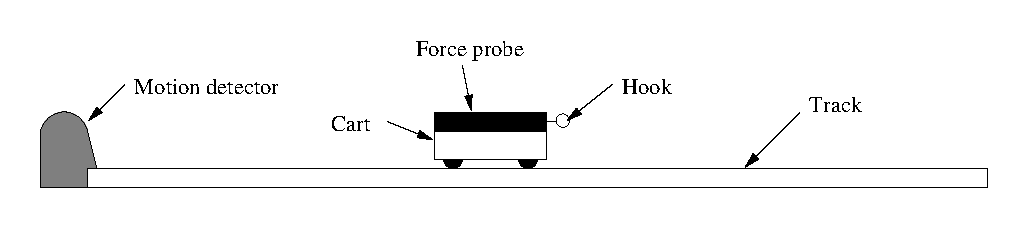
\includegraphics{force1/force1_fig1.eps} \par}


%\caption
%{Equipment setup for qualitative measurements of force and motion.}
%\end{figure}

%\newpage
%(b) Place the cart on the level track.  Suppose you were to grasp the hook on the cart (which %is attached to the force sensor) and move the cart forwards and backwards. Would either the
%velocity or the acceleration graph look like the force graph? Explain. 
%Is either of these motion quantities related to force? 
%That is to say, if you apply a
%changing force to the cart, will the velocity or acceleration change in the
%same way as the force?
\answerspace{20mm}
\pagebreak[3]
(c) To test your predictions, click the \textbf{Record} button, grasp the
hook on the cart and push and pull the cart back and forth 3 or 4 times. Repeat until you get a good run, and adjust the sampling rate and scale of the axes if necessary. Sketch your graphs on the axes below.

%\vspace{-0.3cm}
%{\par\centering 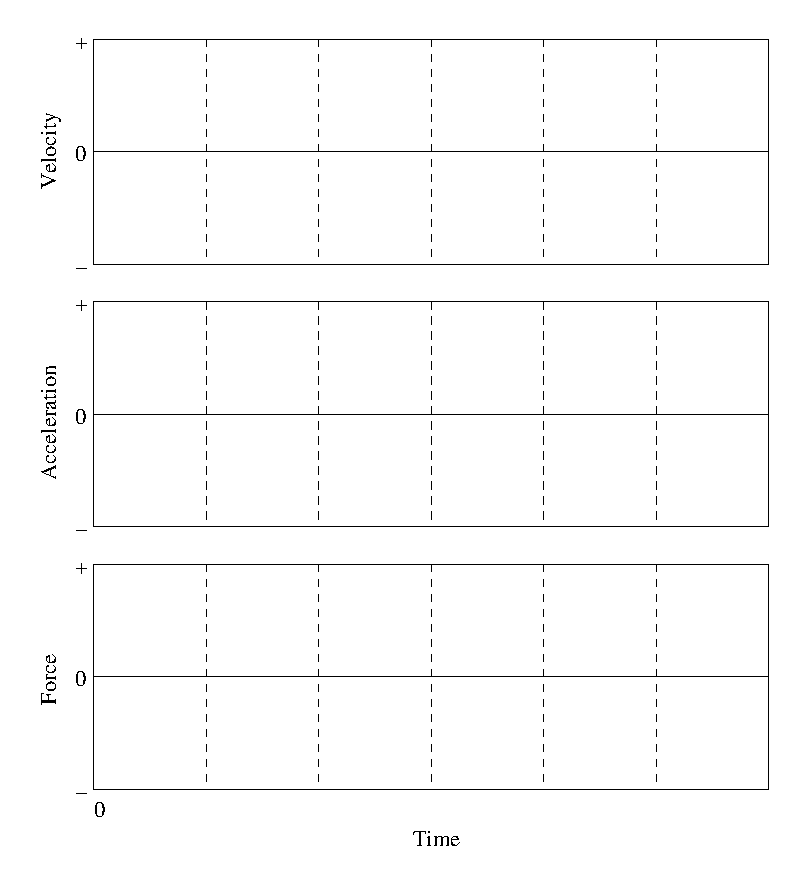
\includegraphics[scale=0.95]{force1/force1_fig2.eps} \par}
%\vspace{-0.4cm}

\begin{lab_groupplot}*{}[lab_grid,
	group style={
		group size=1 by 3,
		xlabels at=edge bottom,
		vertical sep=0.3in,
		},
	width=4.2in,  height=1.4in,
	xlabel=Time (s),
	xmin=0, xmax=12,
	xtick distance = 2, 
	ytick distance = 1, 
	minor tick num=1,
	ytick = {-1,0,1},
	yticklabels = {$-$, 0, $+$},
	]
\nextgroupplot[
	ymin=-1,ymax=1, 
	ylabel={Velocity (m/s)},
	]
\nextgroupplot[
	ymin=-1,ymax=1, 
	ylabel={Acceleration (m/s$^2$)},
	]
\nextgroupplot[
	ymin=-1,ymax=1, 
	ylabel={Force (N)},
	]
\end{lab_groupplot}

(d) Does either graph---velocity or acceleration---resemble the force graph? Which
one? Explain.
\answerspace{15mm}

(e) Based on your observations, does it appear that either the velocity or acceleration
of the cart might be related to the applied force? Explain.
%\answerspace{10mm}
\newpage
\pagebreak[3]
\textbf{Activity 2: Speeding Up }

You have seen in the previous activity that force and acceleration seem to be
related. But just what is the relationship between force and acceleration? 

(a) Suppose you have a cart with very little friction, and that you pull this
cart with a constant force as shown below on the force \textit{vs.}~time graph. Predict with sketches on the axes below the velocity \textit{vs.}~time and acceleration \textit{vs.}~time graphs of the cart's motion.

%\vspace{0.3cm}
%{\par\centering 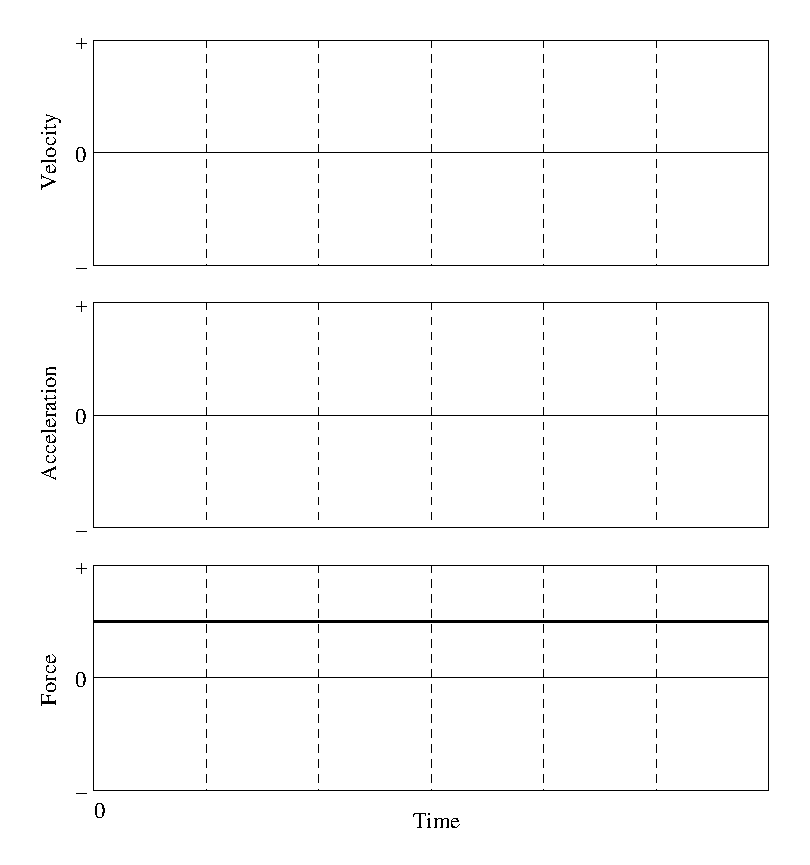
\includegraphics{force1/force1_fig3.eps} \par}
%\vspace{0.3cm}
\begin{lab_groupplot}*{}[lab_grid,
	group style={
		group size=1 by 3,
		xlabels at=edge bottom,
		vertical sep=0.3in,
		},
	width=4.2in,  height=1.4in,
	xlabel=Time (s),
	xmin=0, xmax=12,
	xtick distance = 2, 
	ytick distance = 1, 
	minor tick num=1,
	ytick = {-1,0,1},
	yticklabels = {$-$, 0, $+$},
	]
\nextgroupplot[
	ymin=-1,ymax=1, 
	ylabel={Velocity (m/s)},
	]
\nextgroupplot[
	ymin=-1,ymax=1, 
	ylabel={Acceleration (m/s$^2$)},
	]
\nextgroupplot[
	ymin=-1,ymax=1, 
	ylabel={Force (N)},
	]
\addplot coordinates {(0,0.5) (10,0.5)};
\end{lab_groupplot}

(b) Describe in words the predicted shape of the velocity \textit{vs.}~time and acceleration
\textit{vs.}~time graphs for the cart.
\answerspace{30mm}

%\begin{figure}
\begin{center}
%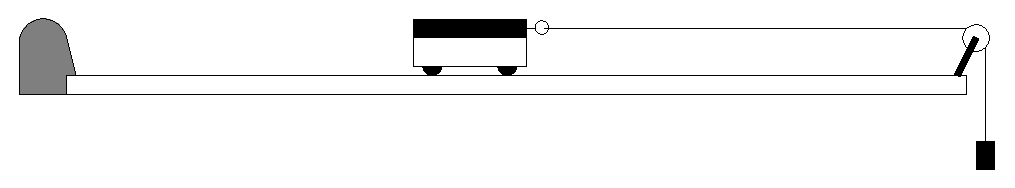
\includegraphics{force1/force1_fig4.eps}
%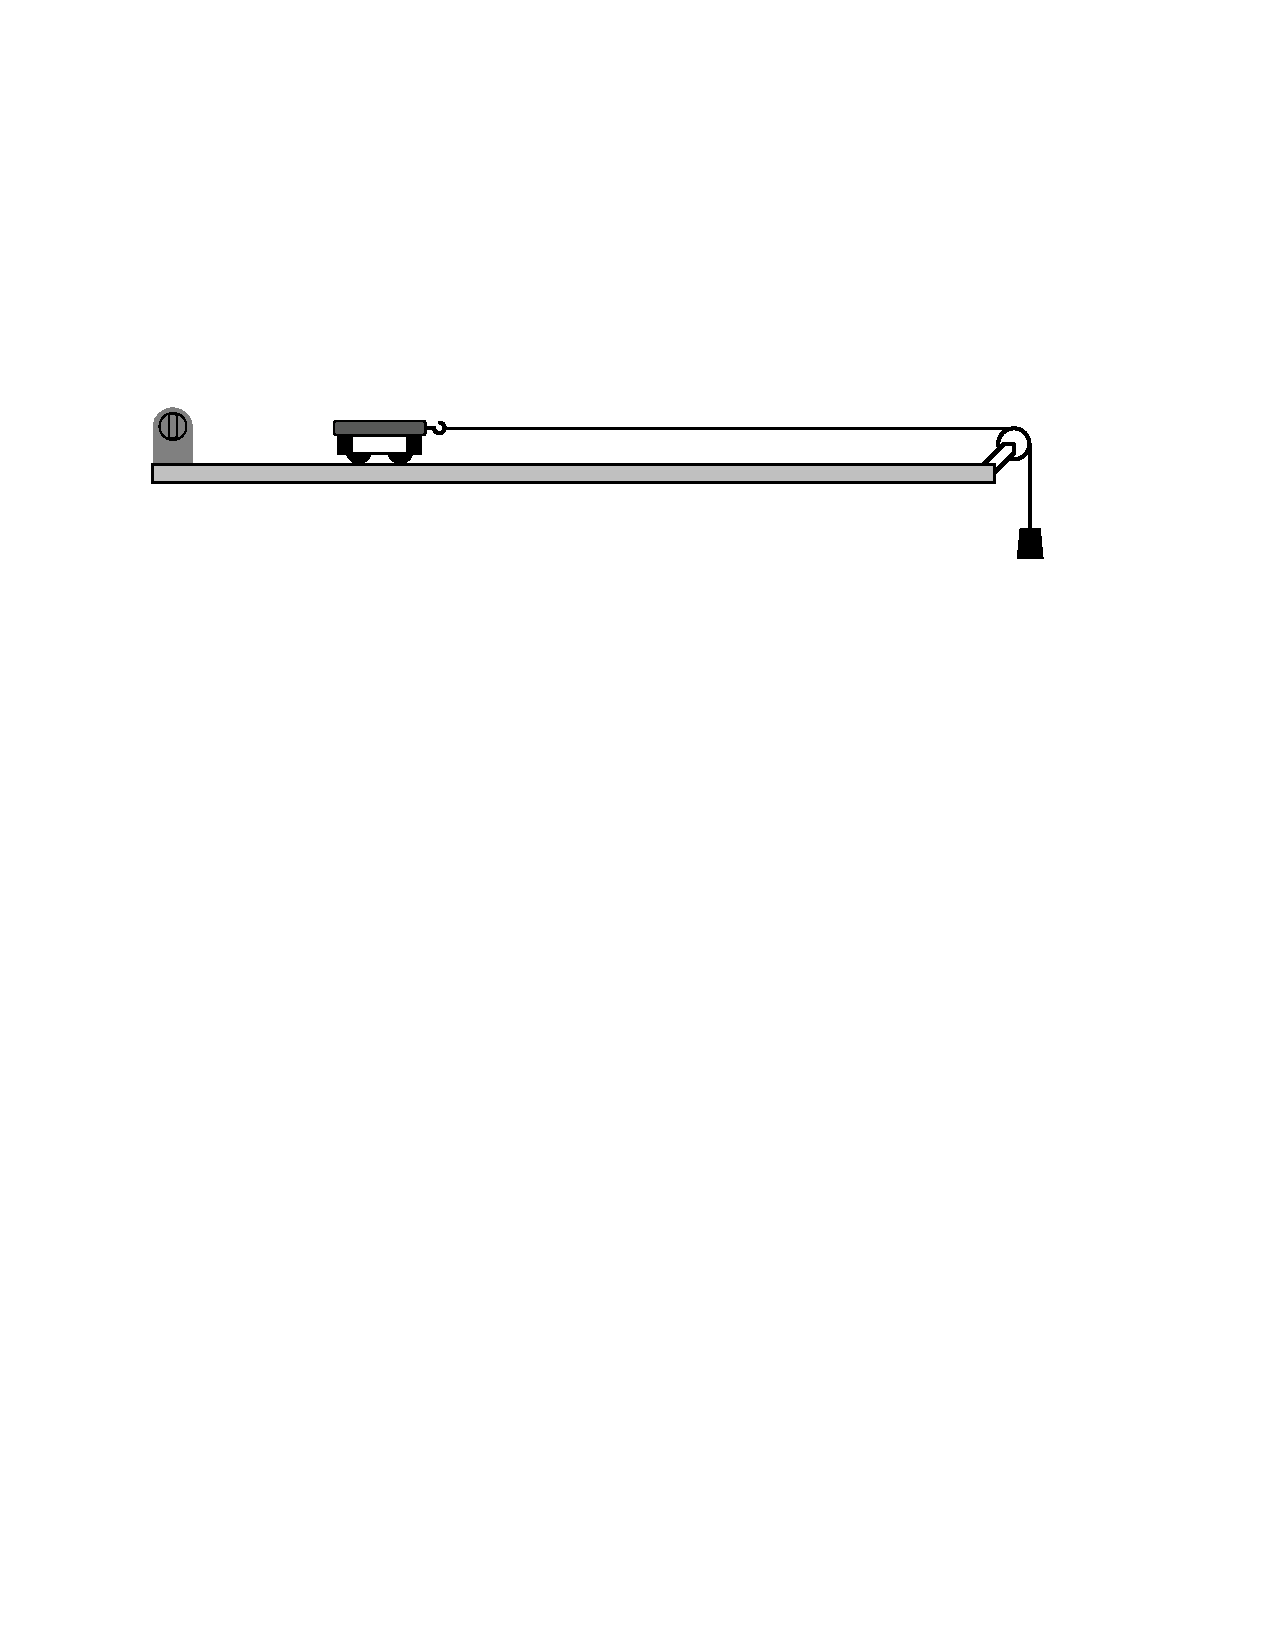
\includegraphics{force1/cart_detector_mass.pdf}
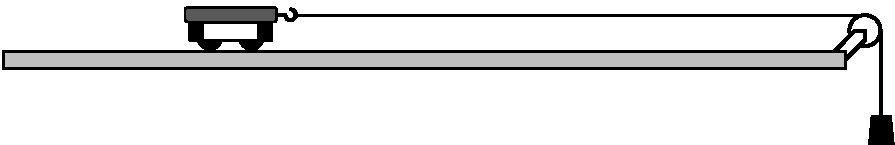
\includegraphics{force1/cart_pulley_mass.pdf}

\vspace{-0.2in}
\textit{Equipment setup for quantitative measurements of force and motion.}
\end{center}
%\end{figure}

(c) Test your predictions. Set up the pulley, cart, and string as shown in the figure above. 
The cart should be the same mass as before. At the start of each trial, tare the cart's built-in force sensor when there is no applied force on the hook.  

Take one of the masses (say, the 50-g one) from the tray and hang it from the end of the string.  Release the cart from rest and create graphs of its motion as it moves in the positive direction (defined by the $x$-axis printed on the top of the cart). Stop the cart before it hits the end of the track. Sketch the graphs neatly on the axes below and indicate the scale on the axes.
%\vspace{0.3cm}
%{\par\centering 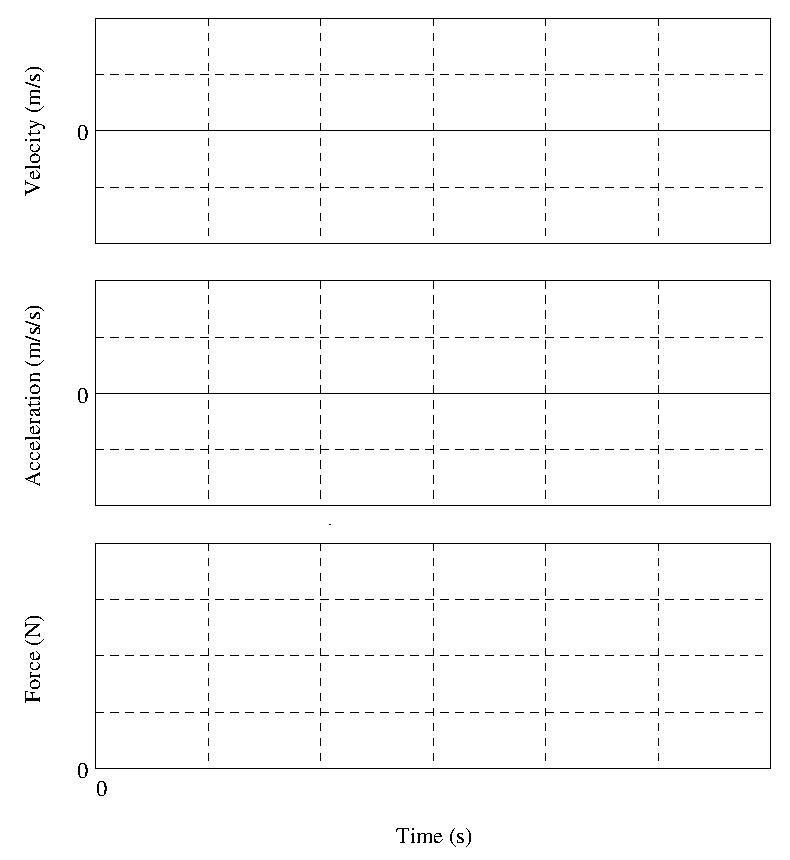
\includegraphics[width=0.65\textwidth]{force1/force1_fig5.eps} \par}
%\vspace{0.3cm}

\begin{lab_groupplot}*{}[lab_grid,
	group style={
		group size=1 by 3,
		xlabels at=edge bottom,
		vertical sep=0.3in,
		},
	width=4.2in,  height=1.4in,
	xlabel=Time (s),
	xmin=0, xmax=12,
	xtick distance = 2, 
	ytick distance = 1, 
	minor tick num=1,
	ytick = {-1,0,1},
	yticklabels = {$-$, 0, $+$},
	]
\nextgroupplot[
	ymin=-1,ymax=1, 
	ylabel={Velocity (m/s)},
	]
\nextgroupplot[
	ymin=-1,ymax=1, 
	ylabel={Acceleration (m/s$^2$)},
	]
\nextgroupplot[
	ymin=-1,ymax=1, 
	ylabel={Force (N)},
	]
\end{lab_groupplot} 

(d) Is the force which is applied to the cart by the string constant, increasing
or decreasing? Explain based on your graph.
\answerspace{15mm}

\pagebreak[2]
(e) How does the acceleration graph vary in time? Does this agree with your
prediction? What kind of acceleration corresponds to a constant applied force?
\answerspace{20mm}

(f) How does the velocity graph vary in time? Does this agree with your prediction?
What kind of velocity corresponds to a constant applied force?
\answerspace{20mm}

(g) Use the \textbf{Highlight} and \textbf{Statistics} functions to determine 
the average force and the average acceleration and record them below. Find the mean values only during the time interval when the force and acceleration are nearly constant. See \textbf{Appendix \ref{capstone}} for details on the use of the \textbf{Highlight} and  \textbf{Statistics} functions of Capstone.
\answerspace{20mm}

\textbf{Activity 3: Acceleration from Different Forces }

In the previous activity you examined the motion of an object with a constant
force applied to it. But, what is the relationship between acceleration and
force? If you apply a larger force to the same object (same mass as before) how
will the acceleration change? In this activity you will try to answer these
questions by applying a different force to the object, and measuring the corresponding
acceleration. 

(a) Suppose you pulled the cart with a force about twice as large as before.
What would happen to the acceleration of the cart? Explain.
\answerspace{20mm}

\pagebreak[3]
(b) Test your prediction by replacing the 50-g hanging mass with a 100-g mass. Tare the force sensor with no force acting on the hook. Now create graphs of the motion as before.  Repeat until you have a good run. Sketch the results on the axes that follow. Don't forget to put the scale on the axes.

%\vspace{0.3cm}
%{\par\centering 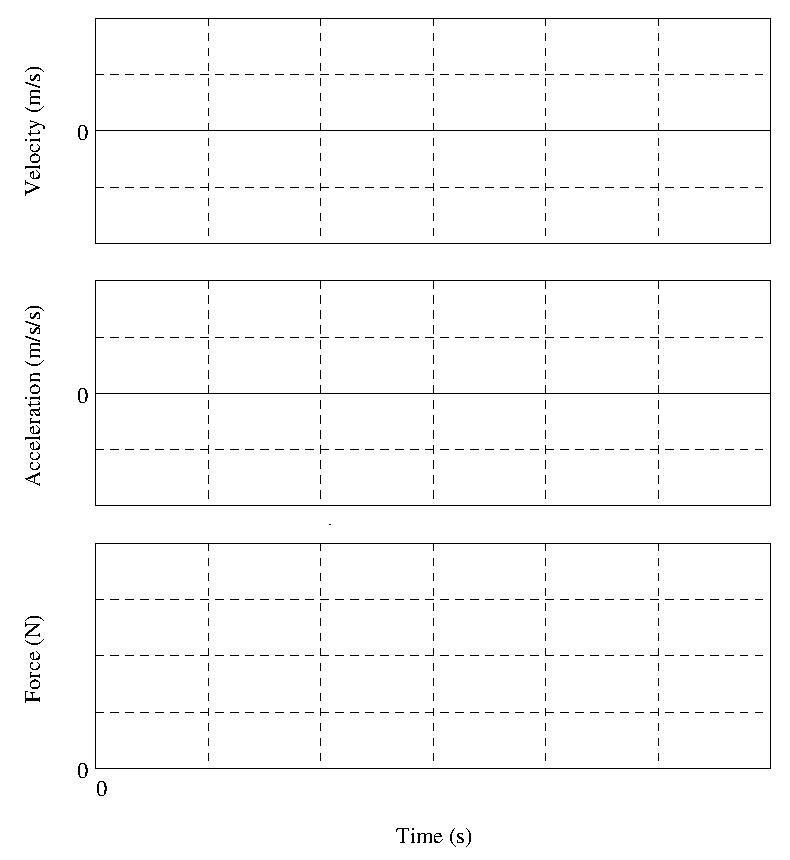
\includegraphics[width=0.65\textwidth]{force1/force1_fig5.eps} \par}
%\vspace{0.3cm}
\begin{lab_groupplot}*{}[lab_grid,
	group style={
		group size=1 by 3,
		xlabels at=edge bottom,
		vertical sep=0.3in,
		},
	width=4.2in,  height=1.4in,
	xlabel=Time (s),
	xmin=0, xmax=12,
	xtick distance = 2, 
	ytick distance = 1, 
	minor tick num=1,
	ytick = {-1,0,1},
	yticklabels = {$-$, 0, $+$},
	]
\nextgroupplot[
	ymin=-1,ymax=1, 
	ylabel={Velocity (m/s)},
	]
\nextgroupplot[
	ymin=-1,ymax=1, 
	ylabel={Acceleration (m/s$^2$)},
	]
\nextgroupplot[
	ymin=-1,ymax=1, 
	ylabel={Force (N)},
	]
\end{lab_groupplot}


(c) Use the \textbf{Highlight} and  \textbf{Statistics} functions to find the 
average force and the average acceleration and record them below. Find the mean values only during the time interval when the force and acceleration are nearly constant.
\answerspace{20mm}

(d) How did the force applied to the cart compare to the force in Activity 2?
\answerspace{20mm}

(e) How did the acceleration of the cart compare to that caused by the force in Activity 2? Did this agree with your prediction? Explain.
\answerspace{20mm}

\pagebreak[2]
\textbf{Activity 4: The Relationship Between Acceleration and Force }

If you accelerate the same object (same mass) with different forces, you can 
plot a graph of force \textit{vs.}~acceleration. You can then find the mathematical relationship between acceleration and force. 

(a) Accelerate the cart with a force roughly midway between the other two forces
tried. Use a hanging mass about midway between those used in the last two activities.
Record the mass below.
\answerspace{10mm}

(b) Graph velocity, acceleration and force. Sketch the graphs on the axes in
Activity 3 using dashed lines.

(c) Find the mean acceleration and force, as before, and record the values in
the table below (in the Activity 4 line). Also, enter the values from the previous 
two activities in the table. Use different combinations of the
masses to get other applied forces and enter the results in the table. 

\vspace{0.3cm}
{\centering \begin{tabular}{|c|c|c|c|}
\hline 
&
Average Force (N)&
Average Acceleration (m/s\( ^{2} \)) &
Mass on string\\
\hline 
Activity 4&
&
&
\\
&
&
&
\\
\hline 
Activity 3&
&
&
\\
&
&
&
\\
\hline 
Activity 2&
&
&
\\
&
&
&
\\
\hline 
Activity 4&
&
&
\\
&
&
&
\\
\hline 
Activity 4&
&
&
\\
&
&
&
\\
\hline 
\end{tabular}\par}
\vspace{0.3cm}

(d) Using \textit{Excel}, plot the average force applied to the cart as a function of the average acceleration of the cart by fitting the data with a linear function. Include a fourth data point (0,0) (since zero force means 0 acceleration). Label and print the graph showing the best fit, and add it to this unit.

(e) Does there appear to be a simple mathematical relationship between the acceleration of the cart (with fixed mass) and the force applied to the cart (measured by the force sensor)? Write down the equation you found and describe the mathematical relationship in words.  What is the slope of the graph?
\answerspace{20mm}

(f) Use the LINEST function in \textit{Excel} (see \textbf{Appendix \ref{excel}: Excel}) to determine the uncertainty in mass of the cart.  Write your result as $m = \overline{m} \pm \Delta m$. Be sure to include proper units.
\answerspace{20mm}

(g) Does your measurement of $m$ from Activity 1 fall within the range indicated in (f) above? If not, what are some possible sources of systematic error?
\answerspace{20mm}

Comment: The relationship which you have been examining between the acceleration of the cart and the applied force is known as Newton's Second Law, \textit{F = ma.}

\pagebreak[2]
\textbf{Homework} 

1. A force is applied which makes an object move with the acceleration shown
below. Assuming that friction is negligible, sketch a force-time graph of the
force on the object on the axes below.

%\vspace{0.3cm}
%{\par\centering 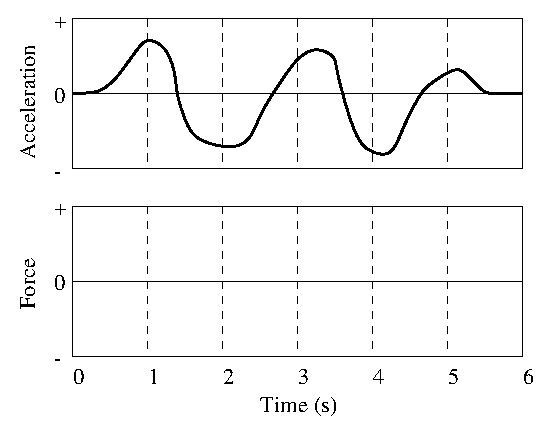
\includegraphics{force1/force1_fig6.eps} \par}
%\vspace{0.3cm}
\begin{lab_groupplot}*{\makegroupverticals[2]{0.5,1,1.5,2}{0}{2.3}}[lab_noticks_2quads,
	group style={group size=1 by 2},
	width=3.0in,  height=1.2in,
	plus_minus_zero_labels,
	xlabel=Time,
	xmin=0,xmax=2.3
	]
\nextgroupplot[ylabel=Acceleration,]
	\addplot +[domain=0:2] {0.8*sin(360*x)};
\nextgroupplot[ylabel=Force,]
\end{lab_groupplot}

Explain your answer:
\vspace{10mm}

2. Roughly sketch the velocity-time graph for the object in question 1 on the
axes below, beginning with a \textit{negative} velocity.  Remember that acceleration 
is the 
\ifForOneTwentyFive
   \textit{slope} 
\else
   \textit{derivative} 
\fi
of velocity.

%\vspace{0.3cm}
%{\par\centering 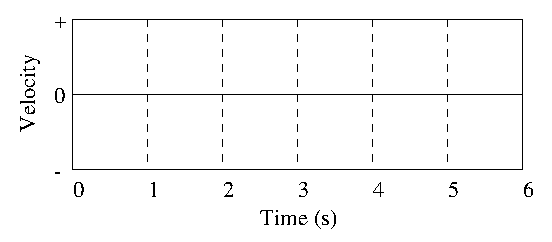
\includegraphics{force1/force1_fig7.eps} \par}
%\vspace{0.3cm}
\begin{lab_groupplot}*{\makegroupverticals[1]{0.5,1,1.5,2}{0}{2.3}}[lab_noticks_2quads,
	group style={group size=1 by 1},
	width=3.0in,  height=1.2in,
	plus_minus_zero_labels,
	xlabel=Time,
	xmin=0,xmax=2.3
	]
\nextgroupplot[ylabel=Velocity,]
\end{lab_groupplot}

3. A cart can move along a horizontal line (the + position axis). It moves with
the velocity shown below.

%\vspace{0.3cm}
%{\par\centering 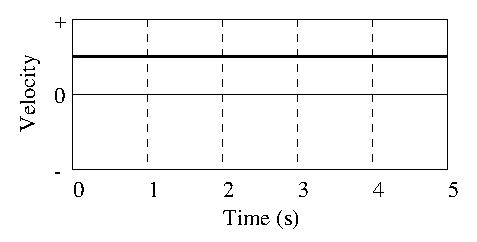
\includegraphics{force1/force1_fig8.eps} \par}
%\vspace{0.3cm}
\begin{lab_axis}*[lab_noticks_2quads,
	width=2.0in,  height=1.2in,
	plus_minus_zero_labels,
	xlabel=Time,
	ylabel=Velocity,
	]
\addplot coordinates {(0,0.6) (0.9,0.6)};
\end{lab_axis}


\pagebreak[2]
Assuming that friction is so small that it can be neglected, sketch on the axes
that follow the acceleration-time and force-time graphs of the cart's motion.

\begin{lab_axis}*[lab_noticks_2quads,
	width=2.0in,  height=1.2in,
	plus_minus_zero_labels,
	xlabel=Time,
	ylabel=Acceleration,
	]
\end{lab_axis}

\begin{lab_axis}*[lab_noticks_2quads,
	width=2.0in,  height=1.2in,
	plus_minus_zero_labels,
	xlabel=Time,
	ylabel=Force,
	]
\end{lab_axis}

%\vspace{0.3cm}
%{\par\centering 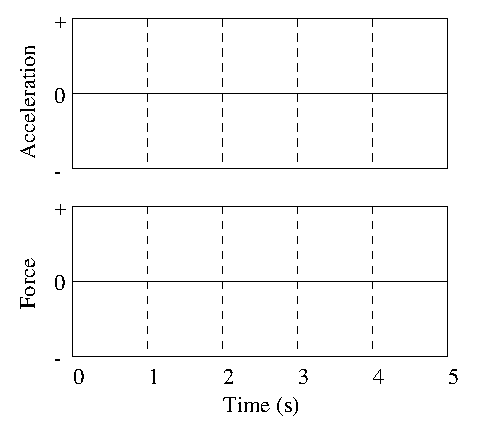
\includegraphics{force1/force1_fig9.eps} \par}
%\vspace{0.3cm}

Explain both of your graphs.
\answerspace{20mm}

Questions 4-6 refer to an object which can move in either direction along a
horizontal line (the + position axis). Assume that friction is so small that
it can be neglected. Sketch the shape of the graph of the force applied to the
object which would produce the motion described. 

4. The object moves away from the origin while speeding up at a constant rate.

%\vspace{0.3cm}
%{\par\centering 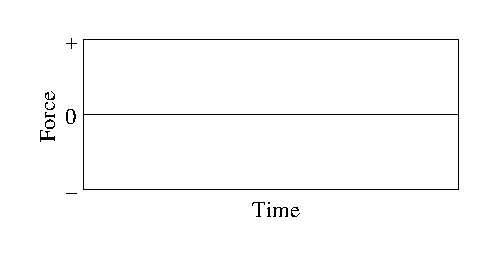
\includegraphics[scale=1.1]{force1/force1_fig10.eps} \par}
%\vspace{0.3cm}
\begin{lab_axis}*[lab_noticks_2quads,
	width=2.0in,  height=1.2in,
	plus_minus_zero_labels,
	xlabel=Time,
	ylabel=Force,
	]
\end{lab_axis}

5. The object moves toward the origin while speeding up at a constant rate.

%\vspace{0.3cm}
%{\par\centering 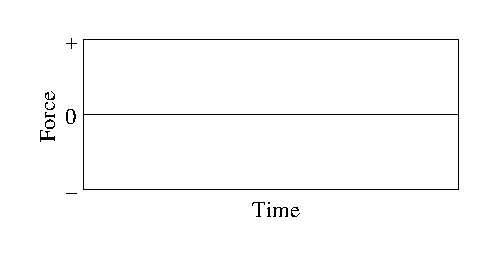
\includegraphics[scale=1.1]{force1/force1_fig10.eps} \par}
%\vspace{0.3cm}
\begin{lab_axis}*[lab_noticks_2quads,
	width=2.0in,  height=1.2in,
	plus_minus_zero_labels,
	xlabel=Time,
	ylabel=Force,
	]
\end{lab_axis}

\pagebreak[2]
6. The object moves away from the origin with a constant velocity.

%\vspace{0.3cm}
%{\par\centering 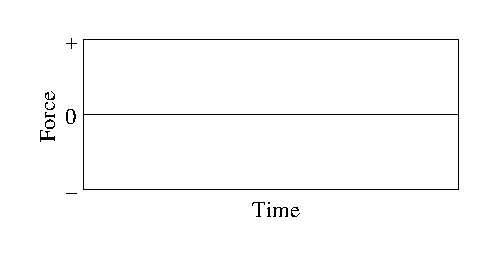
\includegraphics[scale=1.1]{force1/force1_fig10.eps} \par}
%\answerspace{0.3cm}
\begin{lab_axis}*[lab_noticks_2quads,
	width=2.0in,  height=1.2in,
	plus_minus_zero_labels,
	xlabel=Time,
	ylabel=Force,
	]
\end{lab_axis}

Questions 7 and 8 refer to an object which can move along a horizontal line
(the + position axis). Assume that friction is so small that it can be ignored.
The object's velocity-time graph is shown below.

%\vspace{0.3cm}
%{\par\centering 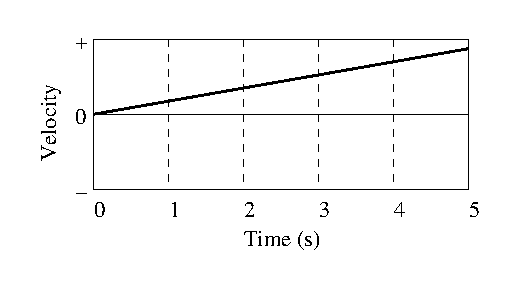
\includegraphics[scale=1.1]{force1/force1_fig11.eps} \par}
%\answerspace{0.3cm}
\begin{lab_axis}*[lab_noticks_2quads,
	width=2.0in,  height=1.2in,
	plus_minus_zero_labels,
	xlabel=Time,
	ylabel=Velocity,
	]
\addplot coordinates {(0,0.0) (0.85,0.8)};
\end{lab_axis}

7. Sketch the shapes of the acceleration-time and force-time graphs on the axes
below.

%\vspace{0.3cm}
%{\par\centering 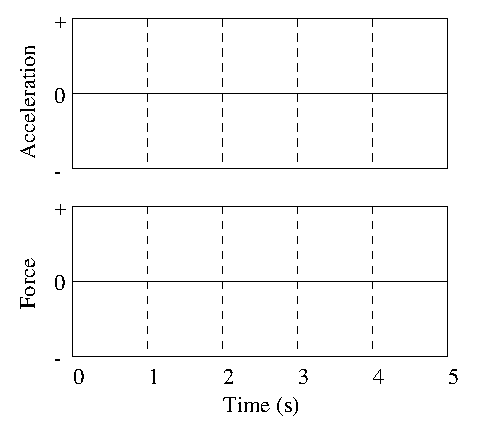
\includegraphics[scale=1.1]{force1/force1_fig9.eps} \par}
%\answerspace{0.3cm}
\begin{lab_axis}*[lab_noticks_2quads,
	width=2.0in,  height=1.2in,
	plus_minus_zero_labels,
	xlabel=Time,
	ylabel=Acceleration,
	]
\end{lab_axis}

\begin{lab_axis}*[lab_noticks_2quads,
	width=2.0in,  height=1.2in,
	plus_minus_zero_labels,
	xlabel=Time,
	ylabel=Force,
	]
\end{lab_axis}

8. Suppose that the force applied to the object were twice as large. Sketch
with dashed lines on the same axes above the force, acceleration, and velocity.
\answerspace{0.3in} %don't really need an answer; just expandable space to make the page look good.

\pagebreak[4]
9.  An object moves along a horizontal line (the +
position axis). Assume that friction is so small that it can be ignored. The
object's velocity-time graph is shown below.

%\vspace{0.3cm}
%{\par\centering 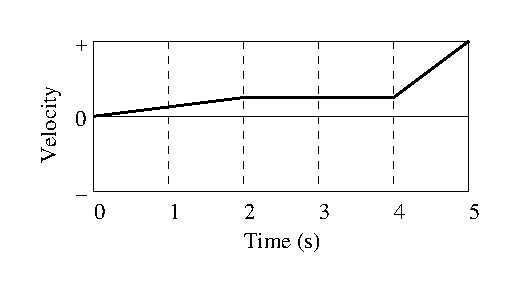
\includegraphics{force1/force1_fig12.eps} \par}
%\vspace{0.3cm}
\begin{lab_groupplot}*{\makegroupverticals[1]{2,4}{0}{5.5}}[lab_noticks_2quads,
	group style={group size=1 by 1},
	width=3.0in,  height=1.5in,
	plus_minus_zero_labels,
	xlabel=Time,
	xmin=0,xmax=5.5
	]
\nextgroupplot[ylabel=Velocity,]
	\addplot coordinates {(0,0) (2,0.3) (4,0.3) (5,0.8)};
\end{lab_groupplot}

Sketch the shapes of the acceleration and force graphs on the axes below.

\begin{lab_groupplot}*{\makegroupverticals[2]{2,4}{0}{5.5}}[lab_noticks_2quads,
	group style={group size=1 by 2},
	width=3.0in,  height=1.2in,
	plus_minus_zero_labels,
	xlabel=Time,
	xmin=0,xmax=5.5
	]
\nextgroupplot[ylabel=Acceleration,]
\nextgroupplot[ylabel=Force,]
\end{lab_groupplot}

%\vspace{0.3cm}
%{\par\centering 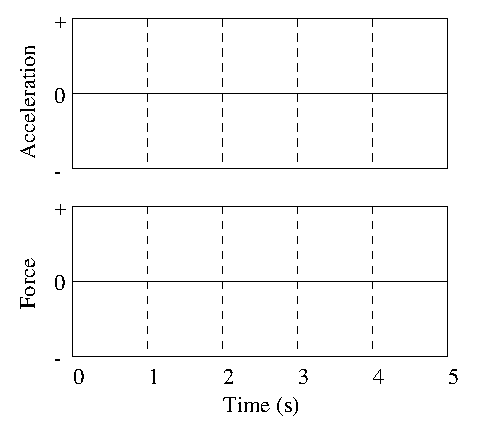
\includegraphics{force1/force1_fig9.eps} \par}
%\vspace{0.3cm}

